\documentclass[a4paper, 12pt]{report}

% these dependencies can be shared between presentation and report
\usepackage[utf8]{inputenc}
%
\usepackage[german]{babel} % References (alternative: ngerman)
%
% ----- Deps -- Styling
\usepackage[scaled]{helvet} % Arial Font
\usepackage{fontawesome} % large icon set
%
% ----- Deps -- Figures and Graphics
\usepackage{graphicx} % embedded images
\usepackage{tikz}
\usetikzlibrary{arrows,shapes,positioning,shadows,trees}
%
% ----- Deps -- Used in Sample Files (Can be defined only in preamble)
\usepackage{qtree} % simple tree generation
\usepackage{pgf-umlsd} % UML like sequence diagrams..
%
% ----- Deps -- Utils
\usepackage{currfile} % https://www.ctan.org/pkg/currfile

% ----- Deps -- References
\usepackage[backend=biber,style=alphabetic]{biblatex}
\usepackage[hidelinks,bookmarks=true]{hyperref}
\addbibresource{bibliography.bib} % import glossary entries

% ----- Deps -- Glossaries
\usepackage[acronym, toc]{glossaries} % https://ctan.org/pkg/glossaries % Load shared Dependencies
\usepackage[hidelinks,bookmarks=true]{hyperref}
%
% ----- Global Variables -------------
\newcommand{\varDocTitle}{Quarterly Report Q1}
\newcommand{\varDocAuthor}{Firstname Lastname}
\newcommand{\varInstitution}{Institution Inc.}
\newcommand{\varAbgabeDatum}{5. Jan 2020}
\newcommand{\varReportType}{Case Study}
%
% ----- Commands -- Import glossary
\makeglossaries
\loadglsentries{glossary}
\glsaddall
%
% ----- Commands -- Use citiations in footnote
\DeclareCiteCommand{\footcite}[\mkbibfootnote] 
	{\usebibmacro{prenote}}                                 
	{\usebibmacro{citeindex}
		\printfield{labelalpha}
		\setunit{\labelnamepunct}
		\printfield[citetitle]{title}
	}
  {\addsemicolon\space}
  {\usebibmacro{postnote}}
%
% ----- Doc -- BEGIN
\begin{document}

    % ----- Doc -- Title Page
    \begin{titlepage}
        \newcommand{\HRule}{\rule{\linewidth}{0.3mm}}
        \center
        \textsc{\large \varInstitution}\\[1.5cm]
        \textsc{\large \varReportType}\\[1.5cm]
        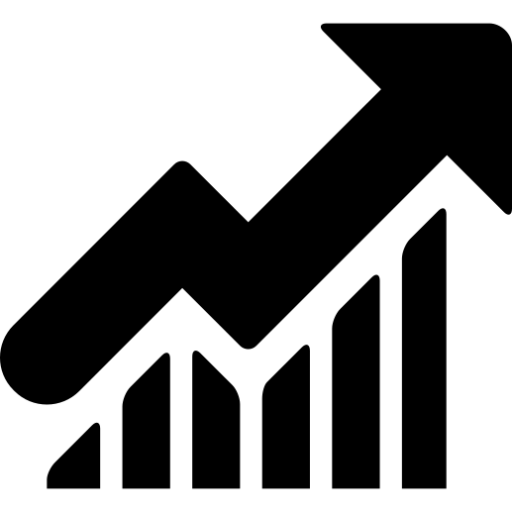
\includegraphics[width=0.5\textwidth]{figures/images/logo.png}\\[1.5cm]
        {\huge \varDocTitle }\\[2cm]
        {\large\textit{Author}}\\
        \textsc{\varDocAuthor}\\[1cm]
        {\large\today\\v1.0}
    \end{titlepage}

    \tableofcontents

    \printglossary
    \printglossary[type=\acronymtype, title=Begriffe und Abkürzungen, toctitle=Begriffe und Abkürzungen]
    
    \listoftables % list of figures
    \listoffigures % list of tables

    \chapter{Images}

    \begin{figure}[!htb]
        \centering
        \includegraphics[scale=0.35]{figures/images/documents.jpg}
        \caption{Image Scaled with factor 0.35}
        \label{fig:mobileid-architecture}
    \end{figure}

    \chapter{Intro}
    \footcite{book:maintainable-software}This line uses a reference from bibliography.bib. You can also use some \gls{mutex} or an acronym from \acrfull{go}.

    \chapter{Figures}

    \section{Trees}

    \subsection{qtree}
    \currfilepath
\vspace{1cm}

\begin{figure}[!htb]
    \centering
    \Tree
    [.e-Government [.e-Democracy [.\textbf{e-Voting} ] ] [.e-Services [.e-Umzug ] [.e-Economy [.easygov ] [.e-MWST  ] ] [.\textbf{e-Identity} [.e-Signatur ] ] [....  ] ] ]
\end{figure}

    \newpage

    \subsection{tikz}
    \currfilepath
\vspace{1cm}

\tikzset{
  basic/.style  = {draw, text width=3.5cm, drop shadow, font=\sffamily, rectangle},
  root/.style   = {basic, rounded corners=2pt, thin, align=center,
                   fill=teal!25},
  level 2/.style = {basic, rounded corners=6pt, thin,align=center, fill=teal!50,
                   text width=8em},
  level 3/.style = {basic, thin, align=left, fill=green!10, text width=6.5em}
}

\begin{center}
    \begin{tikzpicture}[
        level 1/.style={sibling distance=40mm},
        edge from parent/.style={->,draw},
        >=latex]

        % root of the the initial tree, level 1
        \node[root] {E-Govornment}
        % The first level, as children of the initial tree
        child {node[level 2] (c1) {E-Voting}}
        child {node[level 2] (c2) {E-ID}};

        % The second level, relatively positioned nodes
        \begin{scope}[every node/.style={level 3}]

        \node [below of = c1, xshift=15pt] (c11) {Architektur};
        \node [below of = c11] (c12) {Sicherheit};
        \node [below of = c12] (c13) {Vorfälle};

        \node [below of = c2, xshift=15pt] (c21) {Auth};
        \node [below of = c21] (c22) {Sicherheit};
        \node [below of = c22] (c23) {Vorfälle};

        \end{scope}

        % lines from each level 1 node to every one of its "children"
        \foreach \value in {1,2,3}
        \draw[->] (c1.195) |- (c1\value.west);

        \foreach \value in {1,...,3}
        \draw[->] (c2.195) |- (c2\value.west);

        \end{tikzpicture}
 \end{center}
    \newpage

    \section{Sequence Diagrams}
    \currfilepath
\vspace{1cm}

\begin{center}
    \begin{sequencediagram}
        \renewcommand\unitfactor{0.6} % 0.6 is default scale factor

        \newthread[teal!60]{b}{\faUserMd \ Bürger}
        \newthread[red!20]{p}{\faBuildingO \ Service Provider}
        \newinst[2]{bm}{\faMobile \ 2FA}
        \newinst[2]{i}{\faInstitution \ Identity Provider}

        \begin{call}{b}{Login}{p}{Eingeloggt}
            \begin{call}{p}{Authentifizieren}{i}{Bestätigung}
                \begin{call}{i}{MFA Anfrage}{bm}{Faktor bestätigt}
                    \begin{call}{bm}{Authentifizieren}{b}{Authentifiziert}
                    \end{call}
                \end{call}
            \end{call}
        \end{call}

    \end{sequencediagram}
\end{center}
    \newpage

    \printbibliography
    

\end{document}